\subsection{Méthodes d'accès et de conversion des données (Tools)}
Tools contient tous les outils dont nous avons eu besoin lors de notre projet, qui ne sont pas directement relié au mécanisme de fonctionnement de notre jeu, mais qui permettre de simplifier la création des différentes classes. On peut notamment trouver dans Tools les fichiers (et leur header) suivants :

\begin{itemize}
\item \textbf{Table }: La totalité de nos fichiers sont des tableaux (avec comme délimiteurs '';''). C'est pourquoi il nous a paru essentiel de simplifier la lecture des fichiers en créant une classe qui les lirait. Cette classe est capable d'extraire une ligne, une colonne et surtout de donner un élément à partir de son nom de ligne et de son nom de colonne (surcharge de l'opérateur () car [] ne peut être surchargé qu'avec un argument). Afin de standardiser la saisie, nous avons décidé que la lecture des tableaux donnerait uniquement des chaînes de caractères (et ne chercherait donc pas à donner des nombres). Cette classe nous a posé quelques problèmes lorsque nous avons essayé de l'utiliser en écriture.

\begin{figure}[!h]\centering
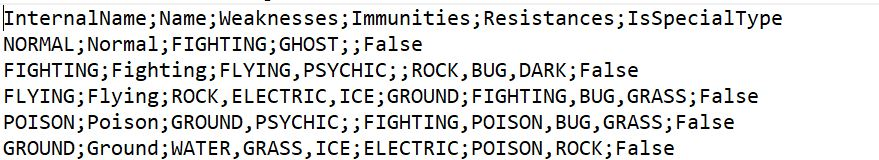
\includegraphics[scale = 0.84]{../Images/fichierTexteExemple.jpg}
\caption{Exemple de fichier lu par Table}
\end{figure}

\item \textbf{VectorMethod} : Ce fichier contient des fonctions supplémentaires concernant les vecteurs. Notamment, un test vector\_in qui permet de dire si un élément est dans le vecteur, et une fonction qui permet de découper les chaînes de caractères. Cette dernière sert par exemple lors de la création des objets de type Table. 
\item \textbf{Conversion} contient une collection de fonctions permettant de convertir les objets d'un type à un autre. En effet, le compilateur MinGW fourni par notre IDE CodeBlocks ne nous laissait pas utiliser les fonction stoi, atoi stol ... qui permettent la conversion directe des types. Nous avons donc créé nos propres fonctions. Ces dernières sont généralement utilisées après la lecture des fichiers contenant des données pour convertir les std::string que la classe Table permet d'extraire (et donc de compenser le fait que Table ne soit composé que de std::string)

\item  \textbf{StatSet} et \textbf{StatSetExt} sont des classes (la seconde héritant de la première) qui permettent de stocker les différentes statistiques de nos Pokémon. Lors de leur création, nous nous sommes aperçus qu'il y avait beaucoup de répétitions d'arguments liés aux points de vie, d'attaque, de défense, d'attaque spéciale, de défense spéciale et de vitesse. Nous avons aussi mis dedans la formule permettant de calculer les statistiques d'un Pokémon. \\
Si on note
\begin{itemize}
\item \textbf{Niv}, le niveau d'un Pokémon, \\
\item \textbf{PV} sa vie maximum, \\
\item \textbf{Stat} la valeur de ses autres statistiques (Attaque Défense, Attaque Spéciale, Défense Spéciale, Vitesse) (cette valeur est celle qui est valable lorsque le Pokémon est soigné), \\
\item \textbf{IV} des paramètres pour chacune des statistiques (ces derniers varient entre 0 et 31, ils sont générés aléatoirement lors de la création d'un Pokémon, ils ne sont ni visibles ni modifiables),\\
\item \textbf{EV} des paramètres pour chacune des statistiques (ces derniers varient entre 0 et 255, ils valent 0 lors de la création d'un Pokémon et varient en fonction des combats effectués, ils ne sont pas visibles par l'utilisateur, mais ce dernier peut les modifier indirectement),\\
\item \textbf{Base} des paramètres pour chacune des statistiques traduisent l'influence de l'espèce sur un Pokémon,
\end{itemize}
alors les statistiques d'un Pokémon sont définies par :
\[
Stat = \Floor{\dfrac{2 * Base + IV + \Floor{\frac{EV}{4}} * Niv + 5}{100} * Nat}
\]
\[
PV =\Floor{\dfrac{2 * Base + IV + \Floor{\frac{EV}{4}} * Niv}{100}} + Niv + 10
\]
\end{itemize}